% !TeX spellcheck = en_GB
\documentclass[a4paper,kul]{kulakarticle} %options: kul or kulak (default)

\usepackage[utf8]{inputenc}
\usepackage[english]{babel}
\usepackage[T1]{fontenc}
\date{Academic year 2023 -- 2024}
\address{
        Bachelor of Engineering Technology \\
        Complex Digital Design (B-KUL-T3WDO2)\\
        Balasch Masoliver Josep}
\title{Lab report Complex Digital Design}
\author{Robbe Decapmaker, Kobe Michiels}
\usepackage{hyperref}
\usepackage{graphicx}
\usepackage{amsmath, amssymb, amsthm}
%\usepackage{siunitx} %cdd_report.tex: error: 18: File `siunitx.sty' not found. \usepackage
\usepackage{flafter}
\usepackage{pdfpages}
\usepackage{pgfplots}
\usepackage{caption}
\usepackage{subcaption}
\usepackage{datetime2}
\usepackage{subfiles}
\usepackage{multicol}
\setlength{\columnsep}{1cm}
\newcommand{\Lapl}{\ensuremath{\mathcal{L}}}

\usepackage{titlesec}
\usepackage[shortlabels]{enumitem}

\setcounter{secnumdepth}{4}

\titleformat{\paragraph}
{\normalfont\normalsize\bfseries}{\theparagraph}{1em}{}
\titlespacing*{\paragraph}
{0pt}{3.25ex plus 1ex minus .2ex}{1.5ex plus .2ex}

\hypersetup{
	pdftitle={Lab report Complex Digital Design},
	pdfsubject={},
	pdfauthor={Robbe Decapmaker, Kobe Michiels},
	pdfkeywords={}
}

\begin{document}

\maketitle
\section{Introduction}

\section{Features}

% A summary of the features of your final project. For the mandatory assignment, you should provide the maximum ADDER_WIDTH tolerated by your design and the number of cycles your design requires to complete a 512-bit addition. If you have completed any of the optional assignments, make sure to summarize them as well in this part.

\section{Technical description}

% A technical description of your main arithmetic designs in the final project. For the improved combinational adder, you should explain the strategy you have followed and provide a high-level diagram of the design. The diagram should be similar to the ones seen in the lectures. For the optional features, you should also provide an explanation and, if required for comprehension, a high-level diagram.

\section{Performance evaluation}

% A performance evaluation of your arithmetic designs, including their worst-case delays (as detailed by Vivado in the post-synthesis report) and the area costs (as detailed by Vivado in the post-synthesis utilization report). 

The performance evaluation of our arithmetic design for an ADDER\_WIDTH of 128 bits consists of an evaluation of the worst-case delay and the area costs. We will firstly generate a post-synthesis Timing Summary to understand if the design met the timing constraints. This Timing Summary is visible on Figure \ref{fig:timing-128-bit}. We get a Worst Negative Slack (WNS) of 0.707 ns. Since this is a positive value, we can conclude that there are no timing errors during synthesis.
\\\\
The Intra-Clock Paths in the Timing Report allow us to form a conclusion about the worst case delay. Using the values from Figure \ref{fig:paths-128-bit}, we can calculate the worst-case delay as the sum of the logic and net delays of the worst path: 1.749 ns + 5.408 ns = 7.157 ns.
\\\\
We can also evaluate the number of clock cycles needed for our addition. The latency of this operation is determined by the division of OPERAND\_WIDTH by ADDER\_WIDTH): OPERAND\_WIDTH/ADDER\_WIDTH = 512/128 = 4 clock cycles.
\\\\
To evaluate the area costs of our design, we take a look at the post-synthesis utilization report on Figure \ref{fig:utilization-128-bit}. We can see that there are 1608 LUTs and 3219 FFs.  

\begin{figure}[h]
	\centering
	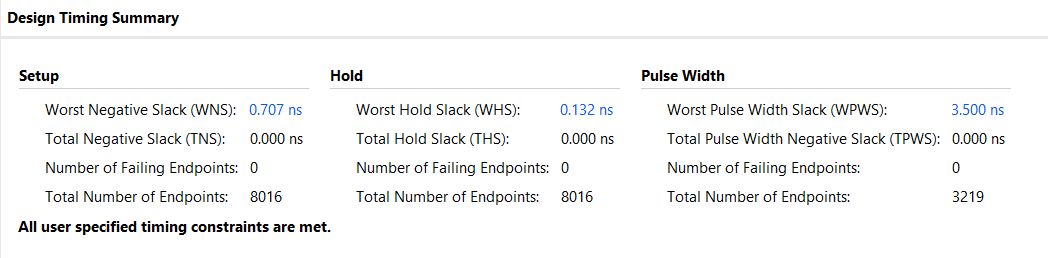
\includegraphics[width=0.75\linewidth]{images/timing-128-bit.png}
	\caption{Design Timing Summary for ADDER\_WIDTH = 128}
	\label{fig:timing-128-bit}
\end{figure}

\begin{figure}[h]
	\centering
	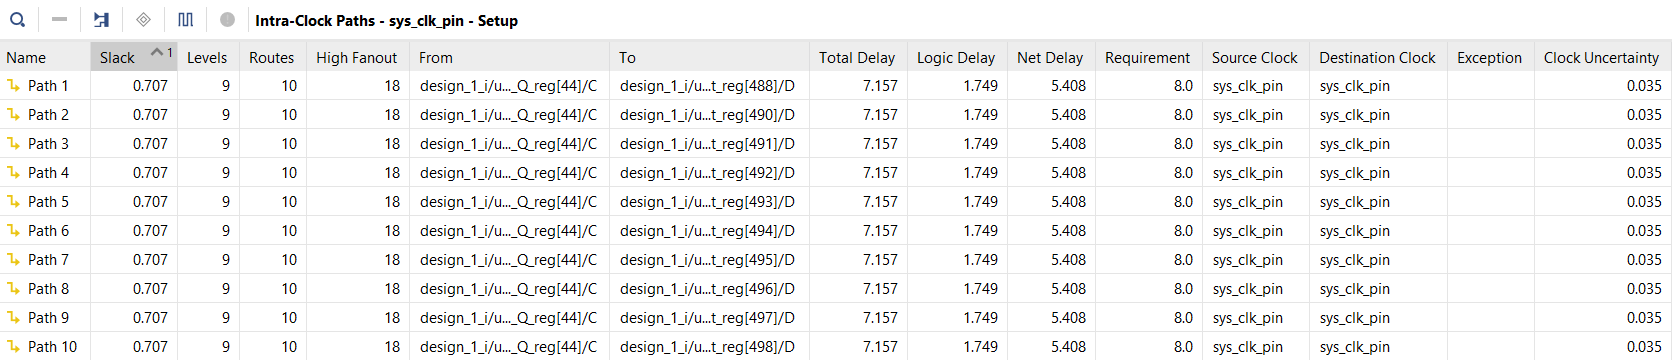
\includegraphics[width=0.75\linewidth]{images/paths-128-bit.png}
	\caption{Intra-Clock Paths for ADDER\_WIDTH = 128}
	\label{fig:paths-128-bit}
\end{figure}

\begin{figure}[h]
	\centering
	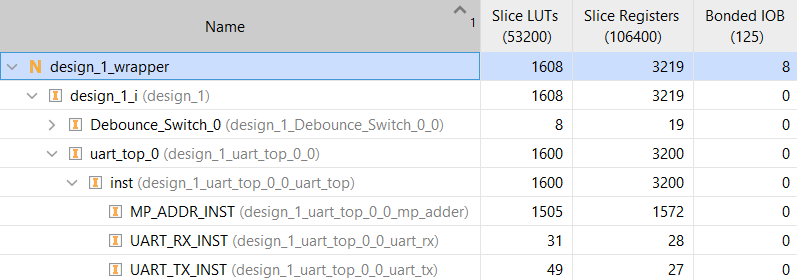
\includegraphics[width=0.75\linewidth]{images/utilization-128-bit.png}
	\caption{Utilization report for ADDER\_WIDTH = 128}
	\label{fig:utilization-128-bit}
\end{figure}

\section{Comparison }

% A comparison of the obtained performance metrics with respect to the original ones from Lab #3, that is, when MP ADDER uses the ripple_carry_adder_Nb with ADDER_WIDTH = 16. Discuss whether the obtained results (speed improvement and area increases) are in line with the expectations.

The reference design from Lab \#3 with an ADDER\_WIDTH of 16 bits has a Worst Negative Slack of 2.651 ns (figure \ref{fig:timing-16-bit}). This is better then our design which has a WNS of 0.707 ns. The worst-case delay of the reference design is 5.213 ns (figure \ref{fig:paths-16-bit}). Our design has a higher one with a value of 7.157 ns. Our design also has a higher area cost, with 1608 LUTs opposed to 1433 LUTs for the reference design (figure \ref{fig:utilization-16-bit}). However, both designs utilize 3219 FFs. 
\\\\
The higher WNS, worst-case delay and area cost is something we expected. Like we can see on figure \ref{fig:128bit-adder}, our design consists of significantly more adders and multiplexers. This will lead to bigger area utilisation and longer paths. These longer paths are the reason for the higher worst-case delay.
\\\\
The latency of the operation of the reference design is equal to 32 clock cycles. This is 8 times more than the latency of our operation. This is also something we expected because our ADDER\_WIDTH is 8 times higher. This increase in ADDER\_WIDTH results in a decrease in iterations and hence, a decrease in clock cycles.

\begin{figure}[h]
	\centering
	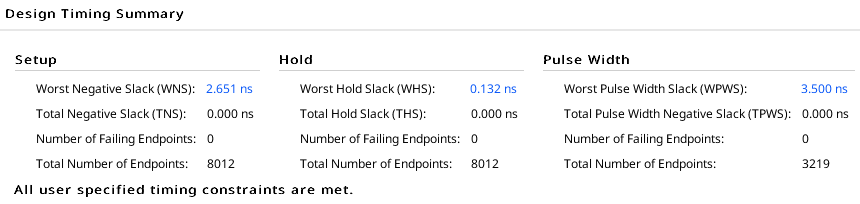
\includegraphics[width=0.75\linewidth]{images/timing-16-bit.png}
	\caption{Design Timing Summary for ADDER\_WIDTH = 16}
	\label{fig:timing-16-bit}
\end{figure}

\begin{figure}[h]
	\centering
	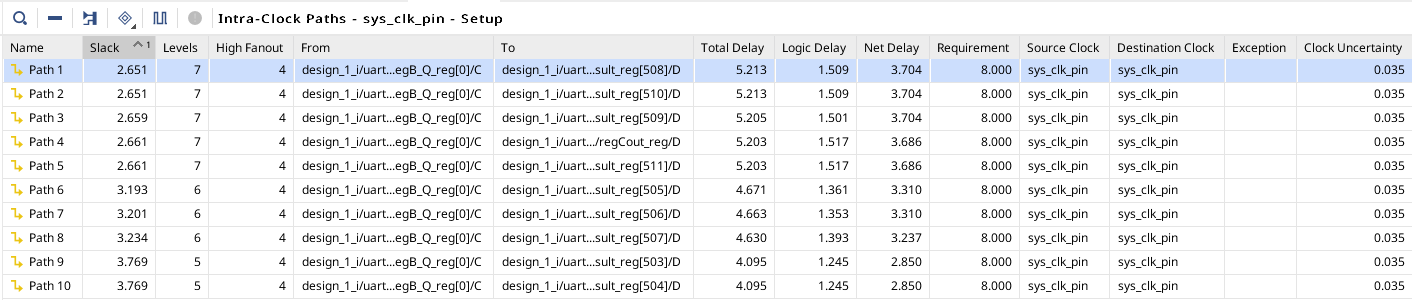
\includegraphics[width=0.75\linewidth]{images/paths-16-bit.png}
	\caption{Intra-Clock Paths for ADDER\_WIDTH = 16}
	\label{fig:paths-16-bit}
\end{figure}

\begin{figure}[h]
	\centering
	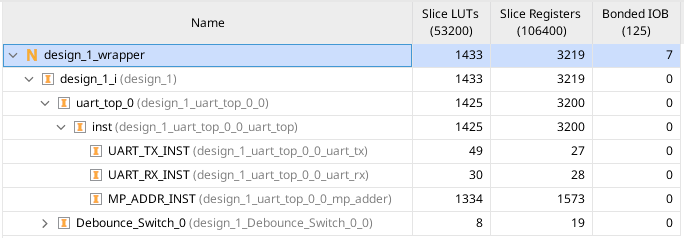
\includegraphics[width=0.75\linewidth]{images/utilization-16-bit.png}
	\caption{Utilization report for ADDER\_WIDTH = 16}
	\label{fig:utilization-16-bit}
\end{figure}

\section{Conclusion}

\end{document}

